% \documentclass[final]{IEEEtran}
\documentclass[letterpaper, 10 pt, journal, twoside]{IEEEtran}

% *** GRAPHICS RELATED PACKAGES ***
%
\ifCLASSINFOpdf
  \usepackage[pdftex]{graphicx}
  \usepackage[export]{adjustbox}
  \usepackage[hidelinks]{hyperref}
  \hypersetup{pdfauthor=author}
  \usepackage{amsmath,amsthm,amsfonts,amssymb}
  \usepackage{pifont}
  \usepackage{cuted}
  \usepackage{multirow}
  \usepackage{enumitem}
  \usepackage{balance}
  \usepackage{subcaption}
  \usepackage{cite}
  \usepackage[linesnumbered,ruled,vlined]{algorithm2e}
  \usepackage{orcidlink}
  \usepackage{soul}
  \usepackage{nomencl}
  
  \makenomenclature

  \newtheorem{theorem}{Theorem}
  \newtheorem{definition}{Definition}

  \usepackage{array}
  \newcommand{\PreserveBackslash}[1]{\let\temp=\\#1\let\\=\temp}
  \newcolumntype{C}[1]{>{\PreserveBackslash\centering}m{#1}}
  \renewcommand{\arraystretch}{1.5}
  
  \newcommand{\cmark}{\ding{51}}%
  \newcommand{\xmark}{\ding{55}}%
\else

  \usepackage[dvips]{graphicx}
\fi

% correct bad hyphenation here
\hyphenation{op-tical net-works semi-conduc-tor}

\begin{document}
\title{MPPDC: Model Prediction-based Perceptual Deformation Control for Multiple Robots\\in Narrow Space Environments
}


\author{Duy-Nam Bui\orcidlink{0009-0001-0837-4360}, Manh Duong Phung\orcidlink{0000-0001-5247-6180}~\IEEEmembership{Senior Member,~IEEE}, and Hung Pham Duy\orcidlink{0000-0001-7878-9409}~\IEEEmembership{Member,~IEEE}% <-this % stops a space
\thanks{\textit{Corresponding author: Hung Pham Duy}}
\thanks{Duy-Nam Bui and Hung Pham Duy are with the VNU-University of Engineering and Technology, Hanoi, Vietnam. {\tt\footnotesize duynam@ieee.org; hungpd@vnu.edu.vn}}
\thanks{Manh Duong Phung is with the Fulbright University Vietnam, Ho Chi Minh City, Vietnam. {\tt\footnotesize duong.phung@fulbright.edu.vn}}
\thanks{Duy-Nam Bui was funded by the Master, PhD Scholarship Programme of Vingroup Innovation Foundation (VINIF), code VINIF.2023.Ths.088.}
\thanks{Code: {\tt\url{https://github.com/duynamrcv/mppdc}}}
\thanks{Video: {\tt\url{https://youtu.be/qW8N0WVQAwU}}}
}

% The paper headers
\markboth{IEEE Transactions on Aerospace and Electronic Systems. Preprint Version.}{Duy-Nam Bui \MakeLowercase{\textit{et al.}}: MPPDC} 


% make the title area
\maketitle


%%%%%%%%%%%%%%%%%%%%%%%%%%%%%%%%%%%%%%%%%%%%%%%%%%%%%%%%%%%%%%%%%%%%%%%%%%%%%%%%
\begin{abstract}
Formation control plays a key role in multi-robot systems, in which a group of robots is coordinated to enhance task performance. Ensuring the safety of robot formations in clustered environments, especially in narrow space environments, remains a significant challenge. This paper proposes a Model Prediction-based Perceptual Deformation Control (MPPDC) strategy for a multi-robot swarm. The strategy proactively ensures the safety of robot formations moving through narrow space by changing the shape according to the environment observed from local sensors. The formation navigation method is modeled as objective functions that express the requirements, constraints, and limitations of the system in the formation movement mission. Additionally, a perceptual deformation strategy is also proposed for distributed decision-making. Finally, simulations, comparisons, and software-in-the-loop testing results are provided to demonstrate the effectiveness of the proposed approach.
\end{abstract}

\begin{IEEEkeywords} multi-robot system, distributed deformation  control, model predictive control, narrow space environments.
\end{IEEEkeywords}

%%%%%%%%%%%%%%%%%%%%%%%%%%%%%%%%%%%%%%%%%%%%%%%%%%%%%%%%%%%%%%%%%%%%%%%%%%%%%%%%
\IEEEpeerreviewmaketitle
% \section*{Supplementary materials}
% Source code: {\tt\small\url{https://github.com/duynamrcv/mppdc}}

% Video: {\tt\small\url{https://youtu.be/qW8N0WVQAwU}}

% \input{nomenclatures}
\section{Introduction}
Unmanned aerial vehicles (UAVs) has gained significant attention in recent years due to their potential applications in various fields, including surveillance, search and rescue operations, and infrastructure inspection~\cite{8682048,9990164}. One crucial aspect of UAV operations is their ability to navigate and maintain formations effectively, especially in complex environments with obstacles. The formation control of multiple UAVs thus plays a vital role in achieving coordination and efficient mission execution~\cite{Anderson,9990236}.

Formation control in multi-robot systems refers to the coordination and control strategies used to form, maintain, and transform formations among a group of robots~\cite{736776,Balch2000}. In scenarios with dense obstacles or narrow spaces, UAV formations need to adapt and reconfigure their shape to navigate through or around obstacles~\cite{7487747,Dang2019,8843165}, as described in Figure~\ref{fig:idea}. This self-reconfigurable capability enables the UAVs to overcome challenging terrain, narrow passages, or complex structures, thereby enhancing their maneuverability and overall mission success. One commonly adopted formation shape is the V-shape configuration, which offers advantages in terms of stability, visibility, and aerodynamic efficiency~\cite{Dang2019,Mirzaeinia2019}. In~\cite{Dang2019}, a formation control algorithm is proposed for multi-UAV systems where the UAVs autonomously adjust their positions within a V-shape to avoid collisions with obstacles. In~\cite{8793765}, a splitting and merging algorithm is proposed for multi-robot formations in environments presented by static and dynamic obstacles. The work in~\cite{8594438} presents a switching strategy of a region-based shape controller for a swarm of robots to deal with the obstacle-avoidance problem in complex environments. 

\begin{figure}
    \centering
    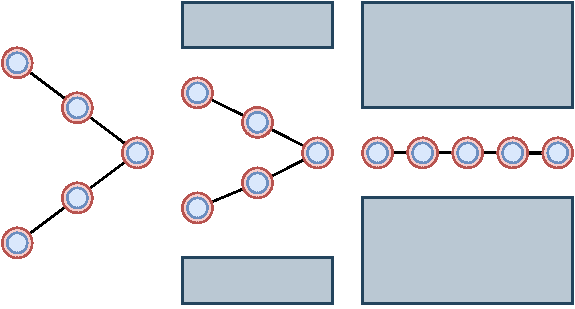
\includegraphics[width=0.6\textwidth]{paper1/images/idea.pdf}
    \caption{The self-reconfigurable V-shape formation can adjust its shape and navigate through narrow passages.}
    \label{fig:idea}
\end{figure}

Recently, advancements in path planning and obstacle avoidance techniques have contributed to the development of self-reconfigurable formation control algorithms. In \cite{8843165}, the angle-encoded particle swarm optimization algorithm is developed for the formation of multiple UAVs used in vision-based inspection of infrastructure. By incorporating constraints related to flight safety and visual inspection, the path and formation can be combined to provide trajectory and velocity profiles for each UAV. The work in \cite{FENG2022} developed a novel optimization method for multi-UAV formation to achieve rapid and accurate reconfiguration under random attacks. In \cite{Gao2022}, multi-UAV reconfiguration problems are modeled as an optimal problem with task assignment and control optimization. However, the focus of their work was on maintaining a fixed formation shape rather than self-reconfiguration in the presence of obstacles.

% \hl{Formation control in environments with obstacles and narrow passages presents challenges in obstacle avoidance, passing through constrained spaces, and so on \cite{Huang2019,Saska2020}. To address these challenges, building a self-reconfiguration formation control strategy is crucial. Such a strategy ensures robustness, adaptability, and efficient navigation, allowing the formation to autonomously adjust its shape to navigate through narrow gaps and avoid obstacles without external intervention. It enhances safety, and mission continuity, making autonomous multi-agent systems more capable and effective in complex and dynamic environments for various applications. Although research efforts have been made in the area of self-reconfigurable formation control, limited work has specifically addressed the challenges of self-reconfigurable formations in large obstacles and narrow environments. }

In this work, we propose a self-reconfigurable V-shape formation control algorithm for multiple UAVs operating in narrow space where the formation cannot maintain its initial shape when moving through this space. The algorithm allows the UAVs to form, maintain and reconfigure the desired V-shape formation by expanding/shrinking its two V-wings to avoid collisions with obstacles and maintain distances among the UAVs. According to the proposed design of distributed behaviors, the V-shape formations can open/close wings or merge into a straight line. Based on it, the UAVs can navigate through narrow passages, bypass obstacles, and optimize their trajectory in accordance to environmental conditions. The main contributions of our work are twofold: (i) develop a self-reconfiguration strategy that can adjust its shape in narrow space environments; and (ii) propose reconfiguration behaviors that navigate UAVs and maintain their shape.

% The remaining sections of this chapter are structured as follows. Section \ref{sec:0design} describes the design of the V-shape formation. Section \ref{sec:0control} presents our implementation of the behavior-based controller. Section \ref{sec:0result} shows simulation results. Our paper ends with conclusions drawn in Section \ref{sec:0conclusion}.
\section{Formation Background}\label{sec:problem}
Consider a swarm $\mathcal{N}$ of $N$ robots labeled $i\in\left\{1,...,N\right\}$. The swarm is modeled as a directed sensing graph $\mathcal{G}=\left(\mathcal{V},\mathcal{E}\right)$, where vertex set $\mathcal{V} = \left\{1,..., N\right\}$ represents the robots, and edge set $\mathcal{E}\subseteq\mathcal{V}\times \mathcal{V}$ includes robot pairs $\left(i, j\right)\in\mathcal{E}$ for which robot $i$ can sense robot $j$. Denote $\mathcal{N}_i=\left\{j\in\mathcal{V}|\left(i,j\right)\in\mathcal{E}\right\}\subset\mathcal{V}$ as the set of $N_i$ neighbors of a robot $i$ in $\mathcal{G}$.

In this work, the dynamics of the robots are represented in discrete time. Denote $p_i(k),v_i(k),u_i(k)\in\mathbb{R}^3$ respectively be the position, velocity and control input of robot $i$ at time $t(k) = k\tau$, where $\tau$ is the sampling period. The robots in the swarm are homogeneous with a body radius $r$. Each robot is equipped with an inertial measurement unit (IMU) to determine its position and orientation, a range sensor to scan the environment, and a wireless ad-hoc network module to carry out peer-to-peer communication with other robots. In this work, the communication delay between each pair of robots is negligible~\cite{AlonsoMora2018,9527169}. The range sensor provides a $360^\circ$ field of view with the scanning area $S_s$ of radius $r_s$, as shown in Figure~\ref{fig:model}. Its point data obtained at time $t(k)$ is represented by set $\mathcal{M}_i(k)=\left\{m\right\}$.
\begin{figure}
    \centering
    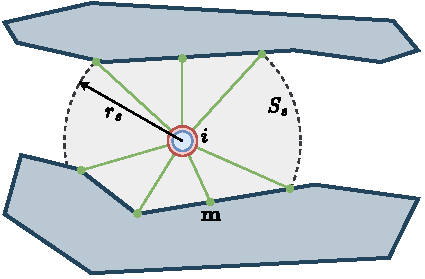
\includegraphics[width=0.48\textwidth]{paper3/images/model.pdf}
    \caption{Illustration of a robot with its range sensor having the scanning area $S_s$ (dashed gray circle) of radius $r_s$ and set $\mathcal{M}_i=\{m\}$ (green) of the acquired point data.}
    \label{fig:model}
\end{figure}

According to~\cite{Soria2021}, the robot in the swarm can be represented as a discrete linear system as follows:
\begin{equation}
    x_i(k+1)=A_ix_i(k) + B_iu_i(k),
\end{equation}
where $A_i$ and $B_i$ are system matrices, $u_i$ is input acceleration, and $x_i=\left[p_i;v_i\right]\in\mathbb{R}^6$ is a state vector including position and velocity. The velocities and accelerations are bounded, i.e., $v_\text{min}\leq v_i(k)\leq v_\text{max}$ and $u_\text{min}\leq u_i(k)\leq u_\text{max}$.
\section{Predictive Reconfiguration Control}\label{sec:propose}

\begin{figure}
    \centering
    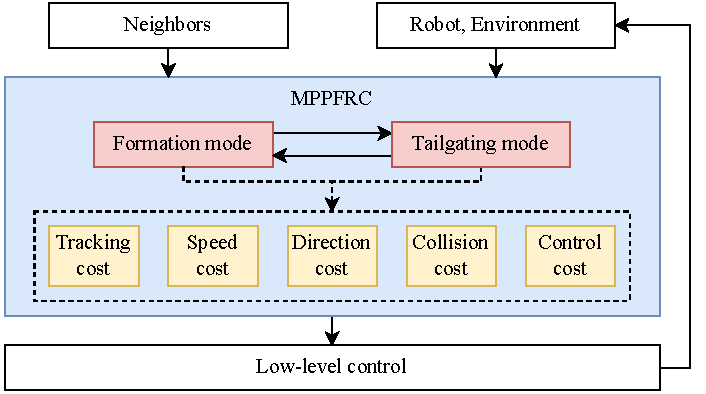
\includegraphics[width=0.7\textwidth]{paper3/images/diagram.pdf}
    \caption{Diagram of the proposed predictive reconfiguration control strategy.}
    \label{fig:diagram}
\end{figure}

The aim of reconfiguration control is to drive the robot swarm through a cluttered environment having narrow passages. The swarm adheres to the following constraints: (\textit{C1}) maintain certain desired shapes; (\textit{C2}) move along a prioritized direction $\mathbf{u}_\text{ref}\in\mathbb{R}^{3}$; (\textit{C3}) obtain the desired speed $\bar{v}_\text{ref}\in\mathbb{R}$; and (\textit{C4}) ensure no collision with other neighbors or obstacles in the environment. To address this problem, we propose a predictive reconfiguration control system as shown in Figure~\ref{fig:diagram}. Inputs to this system include point cloud data from range sensors and the states of neighbor robots. Depending on the environment structure inferred from the point cloud data, the controller operates in either the \textit{``formation''} or \textit{``tailgating''} mode. The \textit{``formation''} mode maintains the desired shape, whereas the \textit{``tailgating''} mode transforms the formation into a line to navigate through narrow spaces like valleys or tunnels. The controller is designed based on a weighted-sum of five cost functions to meet constraints $(C1)-(C4)$. An optimal solver is then used to generate control signals for low-level controllers.

Let $\delta_{ij}\in\mathbb{R}^3,\forall j\in \mathcal{N}_i$ be the vector representing the desired position of robot $i$ with respect to neighbor $j$. The formation is obtained via the following constraint~\cite{Dong2016,6798711}:
\begin{equation}
    \lim_{k\to\infty}{\left(\mathbf{p}_j(k)-\mathbf{p}_i(k)+\kappa\delta_{ij}\right)}=0,\quad\forall i,j\in\{1,...,n\}, i\neq j
\end{equation}
where $\kappa\in[0,1]$ is a scaling factor representing the shrinkage level of the formation. The desired relative position of robot $i$ in the formation is then described as:
\begin{equation}
    \mathbf{p}^*_i(k)=\dfrac{1}{n_i}\sum_{j\in\mathcal{N}_i}{\left(\mathbf{p}_j\left(k\right)+\kappa\delta_{ij}\right)}.
    \label{eqn:formation}
\end{equation}

During the transition between modes, each robot determines a leader as a reference to determine its position. The leader is selected based on the inner product $\tilde{\mathbf{p}}_{ij}$ of the difference between robot $j$ in the neighbor set $\mathcal{N}_i$ and robot $i$, $\mathbf{p}_j-\mathbf{p}_i$, and the desired direction, $\mathbf{u}_\text{ref}$, as follows:
\begin{equation}
    \tilde{\mathbf{p}}_{ij} = \left\langle (\mathbf{p}_j-\mathbf{p}_i),\mathbf{u}_\text{ref}\right\rangle.
    \label{eqn:tildep}
\end{equation}

A positive value of $\tilde{\mathbf{p}}_{ij}$ indicates that robot $j$ is in front of robot $i$ in the $\mathbf{u}_\text{ref}$ direction, and vice versa. Let $\mathcal{P}_i$ be the set of inner products for all robots $j$ in the neighbor set $\mathcal{N}_i$, $\mathcal{P}_i=\left\{\tilde{\mathbf{p}}_{ij}\right\}$. Leader robot ${l_i}$ of robot $i$ is chosen as the closest robot in front of it, i.e.,
\begin{equation}
     l_i=\begin{cases}
    \arg\min_{j}\left\{\tilde{\mathbf{p}}_{ij}\in\mathcal{P}_i\vert\tilde{\mathbf{p}}_{ij}\geq0\right\} & \exists~\tilde{\mathbf{p}}_{ij}\geq0\\ 
    -1 & \text{otherwise}
     \end{cases}
    \label{eqn:li}
\end{equation}

\begin{algorithm}
\caption{Pseudocode of the leader selection}
\label{alg:ls}
\ForEach{$j\in\mathcal{N}_i$}{
    Compute inner product $\tilde{\mathbf{p}}_{ij}$\tcc*[r]{Eq. \ref{eqn:tildep}}
    $\mathcal{P}_i\leftarrow\tilde{p}_{ij}$\;
}
Select leader $l_i$ for robot $i$ to follow\tcc*[r]{Eq. \ref{eqn:li}}
\Return $l_i$\;
\end{algorithm}

Algorithm~\ref{alg:ls} presents the leader selection process. 

In the \textit{``tailgating''} mode, robot~$i$ needs to align and keep a distance~$d_\text{ref}\in\mathbb{R}$ with its leader~$l_i$. This can be formulated as follows:
\begin{equation}
    \lim_{k\to\infty}{\left\Vert \mathbf{p}_{l_i}(k)-\mathbf{p}_i(k)\right\Vert}=d_\text{ref}
    \label{eqn:tailcon}
\end{equation}
The desired relative position of robot~$i$ then can be determined as follows:
\begin{equation}
    \mathbf{p}_i^*(k)= \mathbf{p}_{l_i}(k)-d_\text{ref}\mathbf{u}_\text{ref}.
    \label{eqn:tailgating}
\end{equation}

Using equations \eqref{eqn:tildep} and \eqref{eqn:tailgating}, the formation problem is converted into tracking the desired position $\mathbf{p}_i^*$, which can be handled by predictive controllers. 

\subsection{Predictive control design} 
\begin{figure*}
    \centering
    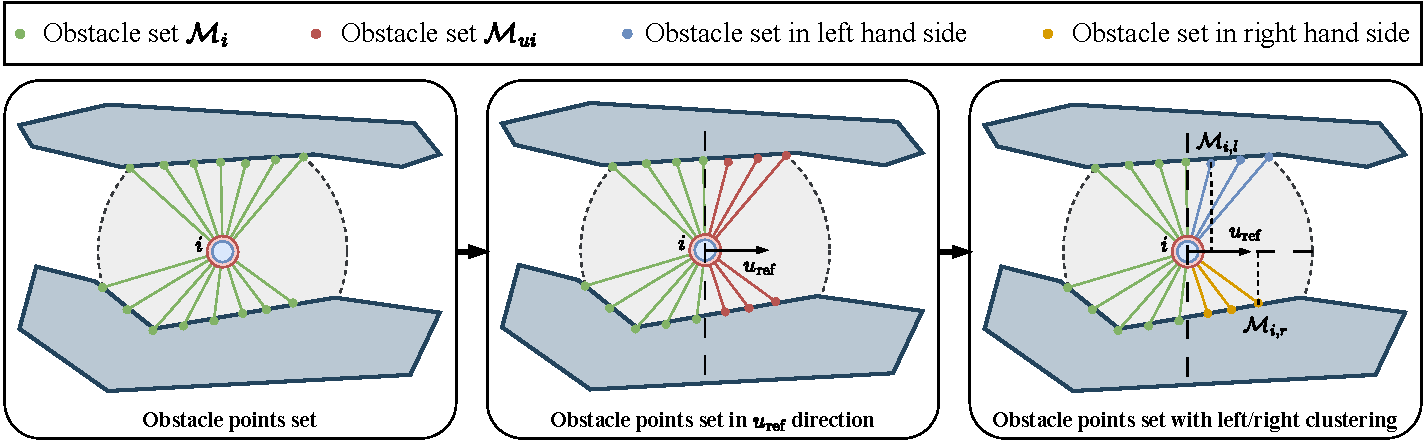
\includegraphics[width=\textwidth]{paper3/images/perception.pdf}
    \caption{The process of estimating the environment's width from the robot's range sensor.}
    \label{fig:perception}
\end{figure*}
The proposed predictive controller uses the desired position $\mathbf{p}_i^*$ as the reference and a set of cost functions to fulfill formation constraints $(C1)-(C4)$. The functions include tracking cost $J_{t,i}$, direction cost $J_{d,i}$, speed cost $J_{s,i}$, obstacle avoidance cost $J_{o,i}$, inter-agent collision cost $J_{i,i}$, and control effort cost $J_{u,i}$. Let $P\in\mathbb{N}^+$ be the prediction horizon, which is finite and shifts forward at each time step; $(\cdot)(k+l|k )$, $l \in\{0,...,P\}$, be the predicted value of $(\cdot)(k+l )$ when the information at time $t(k)$ is available; $\mathbf{X}_i(k)\in\mathbb{R}^{6P}$ be the sequence of the predicted states $\mathbf{x}_i(k+l|k)$ over the horizon $l\in\{1,...,P\}$; and $\mathbf{U}_i(k)\in\mathbb{R}^{3P}$ be the sequence of the predicted control inputs $\mathbf{u}_i(k)$ over the horizon $l\in\{0,...,P-1\}$. The predictive reconfiguration control can be modeled as a non-convex optimization problem as follows:
\begin{equation}
    \min_{\mathbf{U}_i(k)}\left(J_{t,i}(k)+J_{s,i}(k)+J_{d,i}(k)+J_{o,i}(k)+J_{i,i}(k)+J_{u,i}(k)\right)
    \label{eqn:J}
\end{equation}
subject to:
\begin{equation}
    \begin{aligned}
        &\mathbf{x}_i(k+l+1|k)=\mathbf{A}\mathbf{x}_i(k+l|k)+\mathbf{B}\mathbf{u}_i(k+l|k),\\
        &\mathbf{x}_i(k|k)=\mathbf{x}_i(k),\\
        &\mathbf{v}_\text{min}\leq \mathbf{v}_i(k+l|k)\leq \mathbf{v}_\text{max},\\
        &\mathbf{u}_\text{min}\leq \mathbf{u}_i(k+l|k)\leq \mathbf{u}_\text{max},\\
    \end{aligned}
    \label{eqn:constraints}
\end{equation}
with $l\in\{1,...,P\}$, and $i\in\mathcal{N}$. The cost functions are defined as follows.

\subsubsection{Tracking cost}\label{sec:tracking_term}
The tracking term aims to drive the robots toward their reference positions to achieve the desired formation shape. It is defined as the square error between the desired position~$\mathbf{p}_i^*$ and the predicted position~$\mathbf{p}_i$ of robot $i$ as follows:
\begin{equation}
    J_{t,i}(k)=w_t\sum_{l=1}^P{\left\Vert \mathbf{p}^*_i(k+l|k)-\mathbf{p}_i(k+l|k)\right\Vert^2},
\end{equation}
where $w_t$ is a positive tracking weight.

\subsubsection{Speed cost}
The speed cost is used to maintain the desired speed $v_\text{ref}$ of the swarm. It is defined as the squared difference between the actual and the desired speed of the robots as follows:
\begin{equation}
    J_{s,i}(k)=w_s\sum_{l=1}^P\left(\left\Vert \mathbf{v}_i(k+l|k)\right\Vert^2-v_\text{ref}^2\right)^2,
\end{equation}
where $w_s$ is a positive weight.

\subsubsection{Direction cost}
This cost directs the robots to move in the desired direction $\mathbf{u}_\text{ref}$. It is computed based on the normalized dot product between velocity $\mathbf{v}_i$ and the desired direction $\mathbf{u}_\text{ref}$ of robot~$i$. It is equal to zero when the velocity perfectly aligns with the reference direction and otherwise increases proportionally with the degree of misalignment. It is given as follows:
\begin{equation}
    J_{d,i}(k)=w_d\sum_{l=1}^P{\left(1-\dfrac{\left\langle \mathbf{v}_i\left(k+l|k\right),\mathbf{u}_\text{ref}\right\rangle^2}{\left\Vert \mathbf{v}_i(k+l|k)\right\Vert^2}\right)^2},
\end{equation}
where $w_d$ is a positive direction weight.

\subsubsection{Collision avoidance cost}
To avoid collisions, the distance from a robot to any obstacle must be greater than the robot's radius $r$ and the distance between any two robots must be greater than $2r$. Let $d_{ij}=\left\Vert \mathbf{p}_j-\mathbf{p}_i\right\Vert$ be the distance between robots $i$ and $j$, and $d_{im}$ be the distance between robot $i$ and obstacle $\mathbf{m}$. The constraints for collision avoidance  are given as follows:
\begin{equation}
\begin{aligned}
    d_{im}(k+l|k)&\geq r \quad i\in\mathcal{N}, \mathbf{m}\in\mathcal{M}_i(k)
    \label{eq:obsContraint}
\end{aligned}
\end{equation}
\begin{equation}
\begin{aligned}
    d_{ij}(k+l|k)&\geq 2r \quad i\in\mathcal{N},j\in\mathcal{N}_i
    \label{eq:robotContraint}
\end{aligned}
\end{equation}

In this work, constraint (\ref{eq:obsContraint}) is represented via obstacle avoidance cost $J_{o,i}$ defined as a logistic function as follows~\cite{8202163}:   

\begin{equation}
    J_{o,i}(k) = w_o\sum_{l=1}^P \dfrac{1}{1 + \exp{\left(\alpha\left(d_{im}^\text{min}(k+l|k) - r\right)\right)}},
\end{equation}
where $w_o > 0$ is a constant weight, $\alpha > 0$ is a smoothness parameter, and
\begin{equation}
    d_{im}^\text{min}(k+l|k)=\min\left\{d_{im}(k+l|k)|\mathbf{m}\in\mathcal{M}_i\right\}.
\end{equation}

Similarly, constraint (\ref{eq:robotContraint}) is represented via an inter-agent collision cost $J_{i,i}$ defined as follows~\cite{736776}:
\begin{equation}
    J_{i,i}(k)=\dfrac{w_i}{n_i}\sum_{l=1}^P{\sum_{j\in\mathcal{N}_i}}F_{ij}(k+l|k),
\end{equation}
where $w_i>0$ is a constant weight and  
\begin{equation}
    F_{ij}(k+l|k)=\begin{cases}
        0   & \text{if } d_{ij}(k+l|k) \geq \beta r\\
        \dfrac{\beta r-d_{ij}(k+l|k)}{(\beta-2)r}    & \text{if } 2r < d_{ij}(k+l|k) < \beta r\\
        \infty  & \text{if } d_{ij}(k+l|k) \leq 2r
    \end{cases}
\end{equation} 
with $\beta>2$ being the influence ratio of the neighbors.

\subsubsection{Control effort cost}
The control effort cost is used as a penalty term to minimize the control signal. It is defined as:
\begin{equation}
    J_{u,i}(k)=w_u\sum_{l=0}^{P-1}\left\Vert \mathbf{u}_i(k+l|k)\right\Vert^2,
\end{equation}
where $w_u>0$ is a constant control weight.

\subsection{Formation reconfiguration}\label{sec:obs_aware}

Depending on the environment's width, the control system can determine the formation shape and scaling factor $\kappa$. The process of estimating the environment's width is illustrated in Figure~\ref{fig:perception}. Robot $i$ first obtains point cloud data $\mathcal{M}_i$ (green) from its local sensor and then selects a point set $\mathcal{M}_{ui}$ (red) in front of the robot along the moving direction $u_\text{ref}$ as follows:
\begin{equation}
    \mathcal{M}_{ui} = \left\{\mathcal{M}_{i}\vert\left\langle\left(\mathbf{p}_i-\mathcal{M}_{i}\right),u_\text{ref}\right\rangle<0\right\}.
    \label{eqn:mui}
\end{equation}
The DBSCAN algorithm~\cite{10.5555/3001460.3001507} is then used to divide $\mathcal{M}_{ui}$ into two clusters corresponding to the left (blue) and right (yellow) sides of the robot. Data points $\mathcal{M}_{i,l}$ and $\mathcal{M}_{i,r}$ from those clusters with the shortest distance to $u_\text{ref}$ are then selected. Using these points, the environment's width is computed as:
\begin{equation}
    w_e= \left\Vert\left(\mathcal{M}_{i,r}-\mathcal{M}_{i,l}\right)\times \mathbf{u}_\text{ref}\right\Vert
    \label{eqn:we}
\end{equation}
The pseudocode to estimate the environment's width is presented in Algorithm~\ref{alg:we}. 

On the other hand, the formation's width $w_f$ is predefined for each specific formation shape. The scaling factor $\kappa$ then can be computed based on the environment's and formation's width as follows:
\begin{equation}
    \kappa = 
    \begin{cases} 
        \dfrac{w_e - 2r}{w_f} & \text{if } w_e \geq \lambda r \\
        0 & \text{otherwise}
    \end{cases}
    \label{eqn:kappa}
\end{equation}
where $\lambda > 2$ is a scaling coefficient determining the environment's width at which the PRC switches its mode. 

\begin{algorithm}[h!]
\caption{Pseudocode to estimate the environment's width}
\label{alg:we}
Get point set $\mathcal{M}_{ui}$ in front of robot $i$ in moving direction $\mathbf{u}_\text{ref}$\tcc*[r]{Eq. \ref{eqn:mui}}
Cluster $\mathcal{M}_{ui}$ for the left and right sides of the robot using DBSCAN\;
Find point pair $\left(\mathcal{M}_{i,l},\mathcal{M}_{i,r}\right)$, whose distance to $\mathbf{u}_\text{ref}$ is minimum\;
Compute the environment's width $w_e$\tcc*[r]{Eq. \ref{eqn:we}}
\Return $w_e$\;
\end{algorithm}

\begin{algorithm}[h!]
\caption{Pseudocode of the PRC}
\label{alg:our}
Get data point set $\mathcal{M}_i$\;
\If{$\mathcal{M}_i$ is empty}{
    mode $\leftarrow$ \textit{``formation''}\;
    $\kappa \leftarrow 1.0$\;
}
\Else{
    Get the environment's width $w_e$\tcc*[r]{Alg. \ref{alg:we}}
    \If{$w_e$ is None}{
        mode $\leftarrow$ \textit{``formation''}\;
        $\kappa \leftarrow 1.0$\;
    }
    \Else{
        \If{$w_e\leq\lambda r$}{
            mode $\leftarrow$ \textit{``tailgating''}\;
        }
        \Else{
            mode $\leftarrow$ \textit{``formation''}\;
            Estimate the desired formation width $w_f$\;
            \If{$w_e-2r\leq w_f$}{
                Compute the scaling factor $\kappa$\tcc*[r]{Eq. \ref{eqn:kappa}}
            }
            \Else{
                $\kappa\leftarrow1.0$\;
            }
        }
    }
}
\Switch{mode}{
\Case{``formation''}
{
    Get the desired position $\mathbf{p}_i^*$\tcc*[r]{Eq. \ref{eqn:formation}}
}
\Case{``tailgating''}
{
    Select a leader to follow\tcc*[r]{Alg. \ref{alg:ls}}
    Get the desired position $\mathbf{p}_i^*$\tcc*[r]{Eq. \ref{eqn:tailgating}}
}
}
Establish the formation cost function\tcc*[r]{Eqs. \ref{eqn:J}-\ref{eqn:constraints}}

Minimize the cost function to obtain the optimal control signal $\mathbf{u}_i^*$\tcc*[r]{MPC solver~\cite{2020SciPy-NMeth}}

\Return $\mathbf{u}_i^*$\;
\end{algorithm}

Algorithm~\ref{alg:our} presents the pseudocode of the PRC. At each time step, the system estimates the width of the environment to determine the formation mode and the scaling factor $\kappa$. It then computes the desired position $\mathbf{p}_i^*$ for each robot and establishes the formation cost function using equations \eqref{eqn:J} - \eqref{eqn:constraints}. This problem is then solved to find the optimal control signal $\mathbf{u}_i^*$ using common nonlinear programming (NLP)
solvers, such as the Sequential Least Squares Programming (SLSQP)~\cite{kraft1988software}. In this work, we implemented the solver in Python using the optimization software library SciPy~\cite{2020SciPy-NMeth}.
\section{Results}\label{sec4}
\subsection{Simulation and Comparison}
\begin{figure*}[!h]
\begin{subfigure}[b]{\textwidth}
    
    \centering
    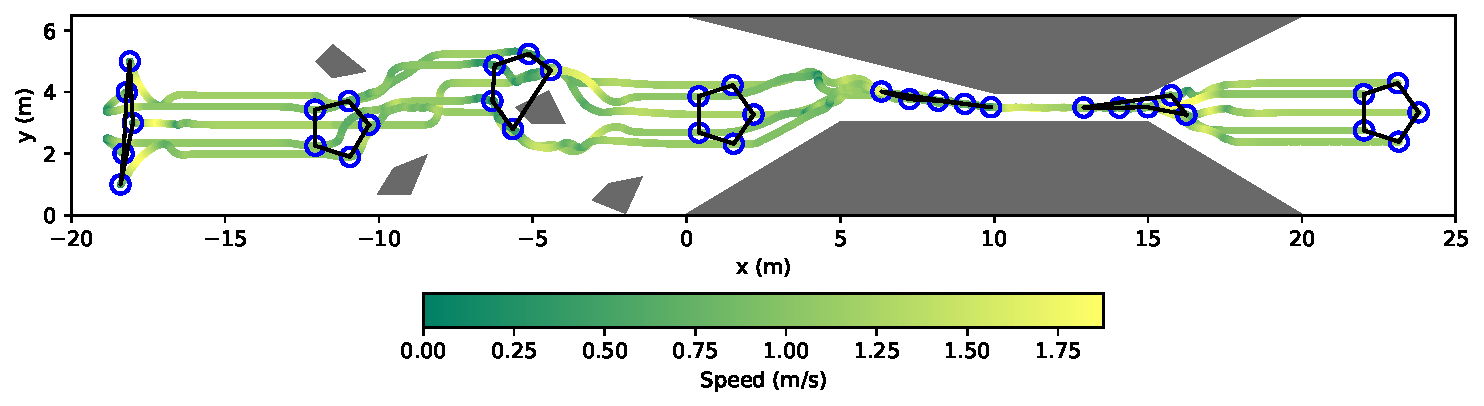
\includegraphics[width=0.9\textwidth]{paper2/images/path_edc_shape1.pdf}
    \caption{Pentagon configuration}
    \label{fig:1path_edc1}
\end{subfigure}
\begin{subfigure}[b]{\textwidth}
    \centering
    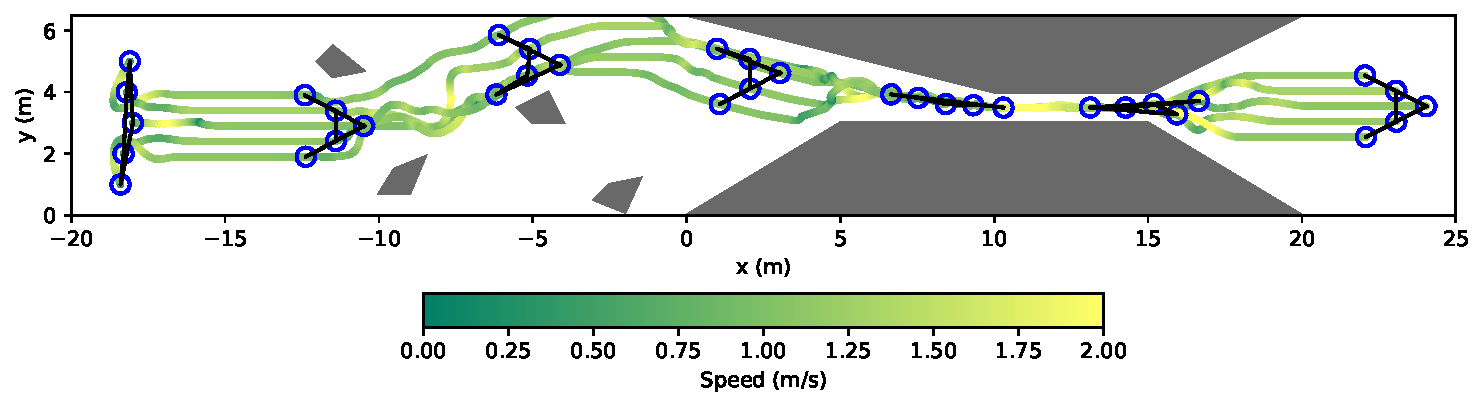
\includegraphics[width=0.9\textwidth]{paper2/images/path_edc_shape2.pdf}
    \caption{V-shape configuration}
    \label{fig:1path_edc2}
\end{subfigure}
\caption{Motion paths and velocity profiles of the proposed \textit{EFRC} strategy in multiple configurations.}
\label{fig:1path}
\end{figure*}

\begin{figure*}[!h]
\begin{subfigure}[b]{0.49\textwidth}
    
    \centering
    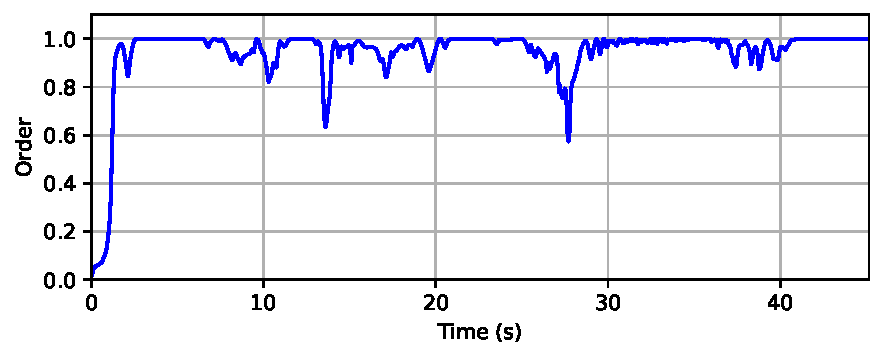
\includegraphics[width=\linewidth]{paper2/images/order_edc_shape1.pdf}
    \caption{Pentagon configuration}
    \label{fig:1order_edc1}
\end{subfigure}
\begin{subfigure}[b]{0.49\textwidth}
    \centering
    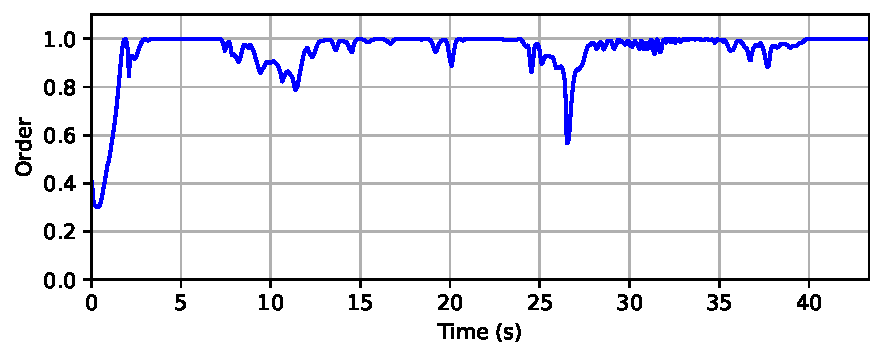
\includegraphics[width=\linewidth]{paper2/images/order_edc_shape2.pdf}
    \caption{V-shape configuration}
    \label{fig:1order_edc2}
\end{subfigure}
\caption{The \textit{order} values of the proposed \textit{EFRC} strategy}
\label{fig:1order}
\end{figure*}

\begin{figure*}[!h]
\begin{subfigure}[b]{0.49\textwidth}
    
    \centering
    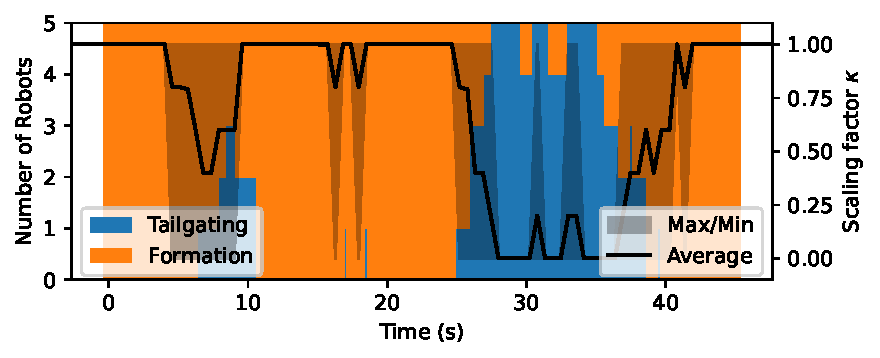
\includegraphics[width=\linewidth]{paper2/images/mode_edc_shape1.pdf}
    \caption{Pentagon configuration}
    \label{fig:1mode_edc1}
\end{subfigure}
\begin{subfigure}[b]{0.49\textwidth}
    \centering
    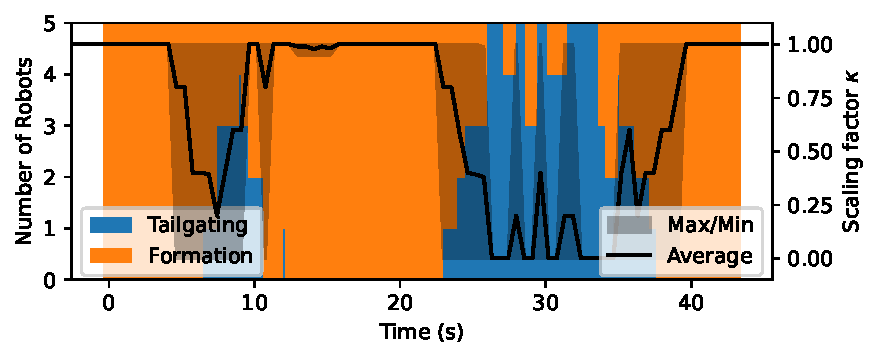
\includegraphics[width=\linewidth]{paper2/images/mode_edc_shape2.pdf}
    \caption{V-shape configuration}
    \label{fig:1mode_edc2}
\end{subfigure}
\caption{Correlation of number of robots and scaling factor of the proposed \textit{EFRC} strategy}
\label{fig:1mode}
\end{figure*}

% The simulations are run on AMD Ryzen 5 5500U with a base frequency of 2.1 GHz. 
The proposed strategy is tested in a complex environment, which consists of 2 areas of different obstacle types, one area is the forest-liked environment, whose obstacle densities is 0.05 obs/m$^2$ (for $-12$~m $<x<0$~m), another area is the width-varying cave-like environment with the most narrowed space is 1~m (for $0$~m $<x<20$~m). The TVF starts randomly from the left-hand side of the environment and has a mission to travel through the confined space to the right-hand side, with the desired direction $u_\text{ref}=\left[1,0,0\right]^T$. We set up a formation with 5 homogeneous robots with two formation configurations, including V-shape and polygon configurations, when the TVF transforms to \textit{``Tailgating''} mode, the desired distance for a robot to follow its leader is set by $d_\text{ref}=1$~m. They have constraints with $v_\text{max}=2$~m/s and $u_\text{max}=2$~m/s$^2$. The control period is set at $\tau=0.1$~s. The comparison is done with pure behavior-based control (\textit{BC})~\cite{736776,Vsrhelyi2018}. For comparison between the different methods, the following performance metrics are used: success rate, mean speed, and mean acceleration cost $(\sum{\left\Vert u(k)\right\Vert^2}/{nT})$, with $T$ is the total travel time of the TVF. The parameters used in both strategies are the same to ensure fairness.

In the simulation, we examined how the \textit{EFRC} guided a TVF to navigate through confined spaces. The motion paths and corresponding velocity profile are presented in Fig.~\ref{fig:1path}. Both two formations, including polygon and V-shape configurations, successfully navigate through confined spaces, which include forest-like and tunnel-like environments. Initially, all robots were on the left-hand side, which did not form the desired configuration. They move in the desired direction and form to the predefined shape. Whenever obstacles are detected, the robot activates the obstacle avoidance behavior, there is no narrow space in the first area, and robots in the formation maintain the \textit{``Formation''} mode. Once narrow space is observed, the TVF transforms to \textit{``Tailgating''} mode, which is assigned itself by each robot observation. The straight line configuration is then created, which can help the formation pass through the gap. When the robot escapes the narrow passage, the mode turns back to \textit{``Formation''} mode, which reforms to the desired configuration. Finally, the formation successfully passes through the confined space. Fig.~\ref{fig:1path} presents the motion paths of the TVF, which are conducted by the proposed strategy in multiple configurations.

To further investigate the effectiveness of the proposed strategy, the \textit{order} $\Phi$ metric is defined to measure the heading disturbance of robots in formation during movement. The order's values are in $\left[0,1\right]$, and if the formation has no heading, the order is close to 1 \cite{Vicsek1995}.
\begin{equation}
    \Phi=\dfrac{1}{n}\left\Vert\sum_{i=1}^n{\dfrac{v_i}{\left\Vert v_i\right\Vert}}\right\Vert
\end{equation}
where $v_i$ is the velocity of robot $i$.

Fig.~\ref{fig:1order} illustrates the order information of the TVF's heading throughout the movement process. The figures reveal that the heading order of the swarm in both two scenarios during movement is satisfactory ($\Phi = 1$), When the formation encounters obstacles, the \textit{order} value is changed but still forms the overall configuration. However, disorderliness in the heading order becomes apparent during the transition from \textit{``Formation''} to \textit{``Tailgating''} and vice versa. This is because the structure of the formation undergoes a significant change, resulting in a disorderly heading order.

Fig~\ref{fig:1mode} describes the correlation between the number of robots in different modes and the scaling factor $\kappa$ to evaluate the effectiveness of the synthesized controllers in the proposed deformation strategy. When the TVF encounters obstacles, the configuration is adapted based on the observation of each robot. As a result, the mode of each robot is different at the same time. Also, the scaling factor $\kappa$ is different between robots in the TVF, due to its position and the observation. In collision-free, all robots in the TVF remain in \textit{``Formation''} mode, which contributes to maintaining the original configuration. On the other hand, when narrow space is detected by all robots, the mode transforms to \textit{``Tailgating''}, which forces robots to the straight line configuration to safely navigate through narrow space. The value of $\kappa=0$ when all robots in the TVF are in the \textit{``Tailgating''} mode.

\begin{table}
\caption{Comparison between \textit{BC} and our method, \textit{EFRC} . Each comparison is over 10 simulations of 5 robots in two different configurations. The metrics displayed in the table are the success rate, mean speed, and mean acceleration cost.}
\label{tbl:com}
\centering
\begin{tabular}{C{3.2cm} C{2.cm} C{2.0cm} C{3.0cm} C{3.0cm}}
\hline\hline
Configuration             & Strategy & Succ. & Mean speed (m/s) & Mean Acc. cost (m$^2$/s$^4$)  \\ \hline
\multirow{2}{*}{Pentagon} & EFRC      & \textbf{10/10}        & 0.6773   & \textbf{3.6873}          \\
                          & BC       & 0/10    & \textbf{0.7785}   & 4.3874      
                          \\ \hline
\multirow{2}{*}{V-shape}  & EFRC      & \textbf{10/10}        & 0.7129   & \textbf{4.0978}          \\
                          & BC       & 0/10   & \textbf{0.8877}      & 4.9402 \\ \hline\hline    
\end{tabular}
\end{table}

To further verify the effectiveness of the proposed strategy against the pure behavioural-based control (\textit{BC})~\cite{736776,Vsrhelyi2018}, Table~\ref{tbl:com} presents a comparison between proposed strategy, \textit{EFRC} and \textit{BC}. It can be seen that the proposed \textit{EFRC} strategy outperforms the \textit{BC} in success rate, which can navigate formation passes through a confined space without any collision. Meanwhile, the \textit{BC} always fails when encountering a narrow space (see Fig.~\ref{fig:1sample}). The mean acceleration cost per time is also smaller than the \textit{BC}, because \textit{BC} costs more energy to deal with the surrounding obstacles. The \textit{EFRC} provides an effective method to deal with obstacles by the adaptation configuration. However, the mean speed of the TVF is slightly smaller than the standard approach, due to the translation mode while moving affect to the speed down of the TVF.

\subsection{Validation on the software-in-the-loop Gazebo}
\begin{figure*}[h!]
    \centering
    \begin{subfigure}[b]{0.45\textwidth}
    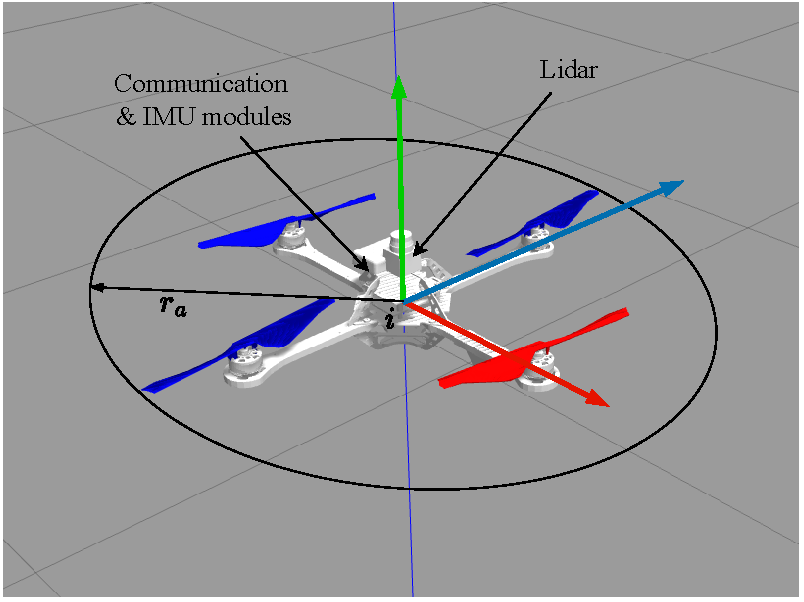
\includegraphics[width=\textwidth]{paper2/images/gazebo_uav.pdf}
    \caption{Gazebo SIL model}
    \label{fig:1gazebo_uav}
    \end{subfigure}
    \begin{subfigure}[b]{0.44\textwidth}
    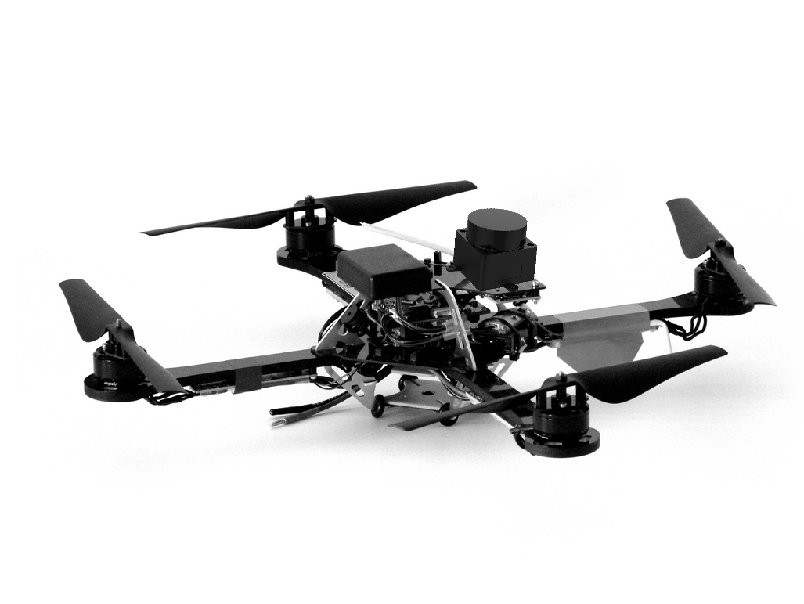
\includegraphics[width=\textwidth]{paper2/images/hummingbird.pdf}
    \caption{Real UAV model \cite{Furrer2016,Bui2022}}
    \label{fig:1gazebo_real}
    \end{subfigure}
    \caption{Used Hummingbird UAV model}
    \label{fig:1gazebo_setup}
\end{figure*}

\begin{figure*}[h!]
    \centering
    \begin{subfigure}[b]{0.495\textwidth}
    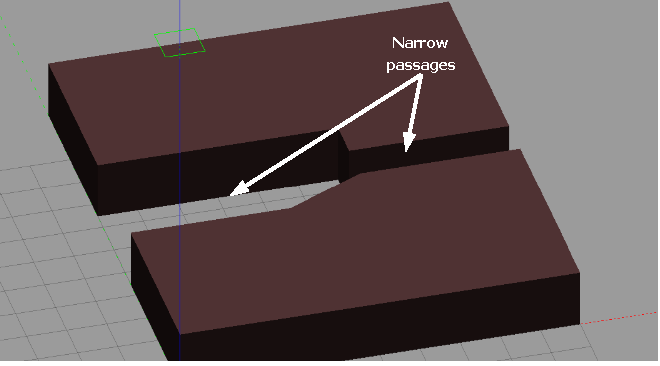
\includegraphics[width=\textwidth]{paper2/images/gazebo_env.pdf}
    \caption{The Gazebo environment}
    \end{subfigure}
    \begin{subfigure}[b]{0.40\textwidth}
    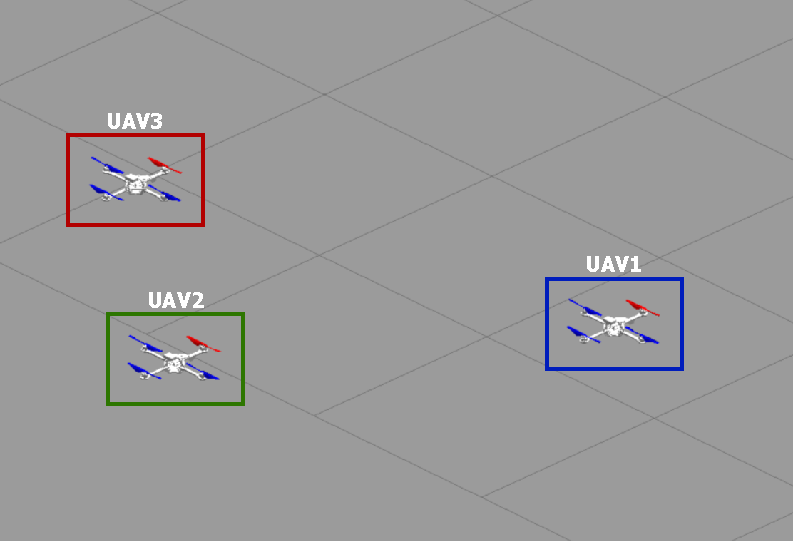
\includegraphics[width=\textwidth]{paper2/images/gazebo_init.pdf}
    \caption{Random initial positions}
    \label{fig:1gazebo_init}
    \end{subfigure}
    \caption{The environment in SIL test}
    \label{fig:1gazebo_env}
\end{figure*}

\begin{figure*}
    \centering
    \begin{subfigure}[b]{0.48\textwidth}
    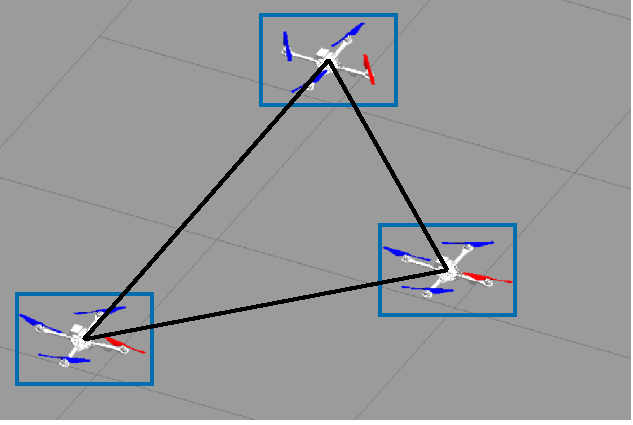
\includegraphics[width=\textwidth]{paper2/images/gazebo_res1.pdf}
    \caption{Maintain triangle formation from random}
    \label{fig:1gazebo_1}
    \end{subfigure}
    \begin{subfigure}[b]{0.48\textwidth}
    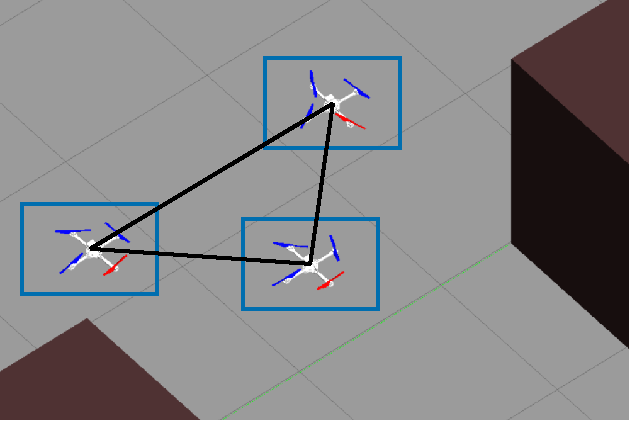
\includegraphics[width=\textwidth]{paper2/images/gazebo_res2.pdf}
    \caption{Small-scaled triangle formation}
    \label{fig:1gazebo_2}
    \end{subfigure}
    \begin{subfigure}[b]{0.48\textwidth}
    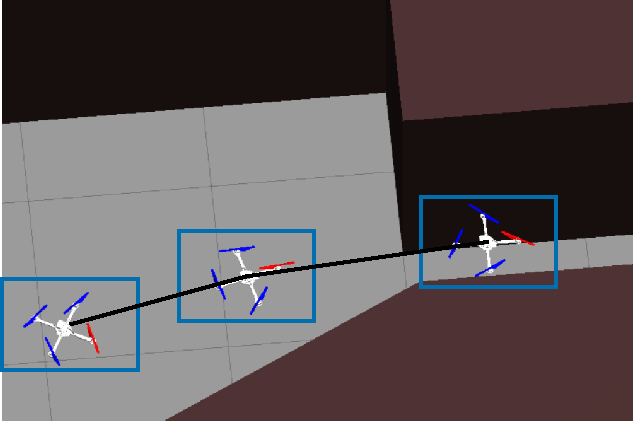
\includegraphics[width=\textwidth]{paper2/images/gazebo_res3.pdf}
    \caption{Transform to line formation}
    \label{fig:1gazebo_3}
    \end{subfigure}
    \begin{subfigure}[b]{0.48\textwidth}
    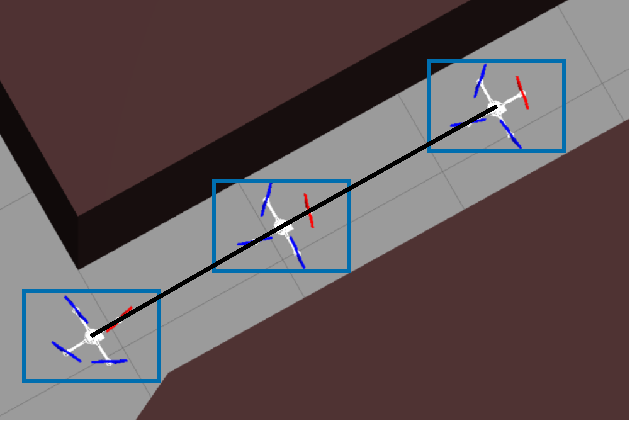
\includegraphics[width=\textwidth]{paper2/images/gazebo_res4.pdf}
    \caption{Line formation}
    \label{fig:1gazebo_4}
    \end{subfigure}
    \begin{subfigure}[b]{0.48\textwidth}
    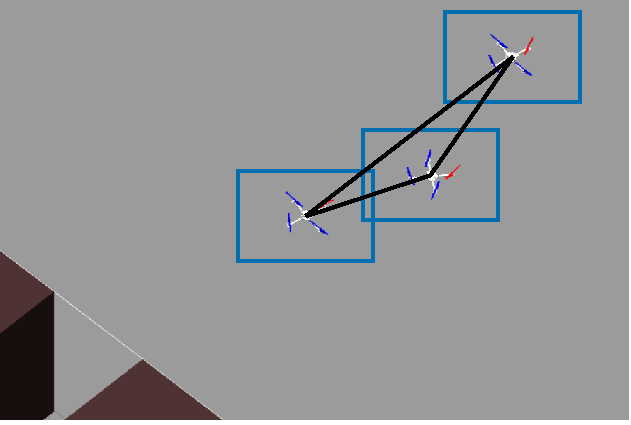
\includegraphics[width=\textwidth]{paper2/images/gazebo_res5.pdf}
    \caption{Transform back to triangle formation}
    \label{fig:1gazebo_5}
    \end{subfigure}
    \begin{subfigure}[b]{0.48\textwidth}
    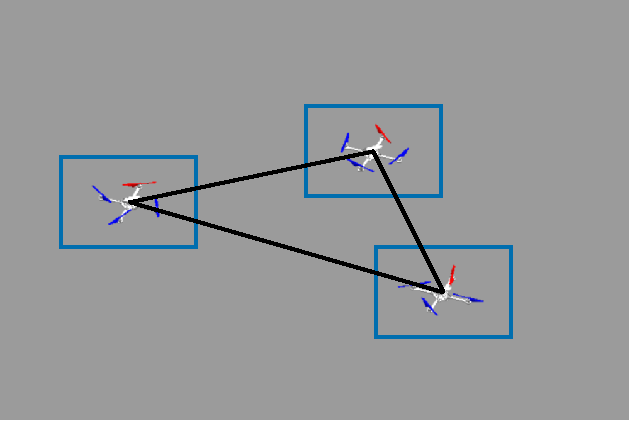
\includegraphics[width=\textwidth]{paper2/images/gazebo_res6.pdf}
    \caption{Original triangle formation}
    \label{fig:1gazebo_6}
    \end{subfigure}
    \caption{Validation results captured in the SIL Gazebo}
    \label{fig:1gazebo_result}
\end{figure*}

\begin{figure*}
    \centering
    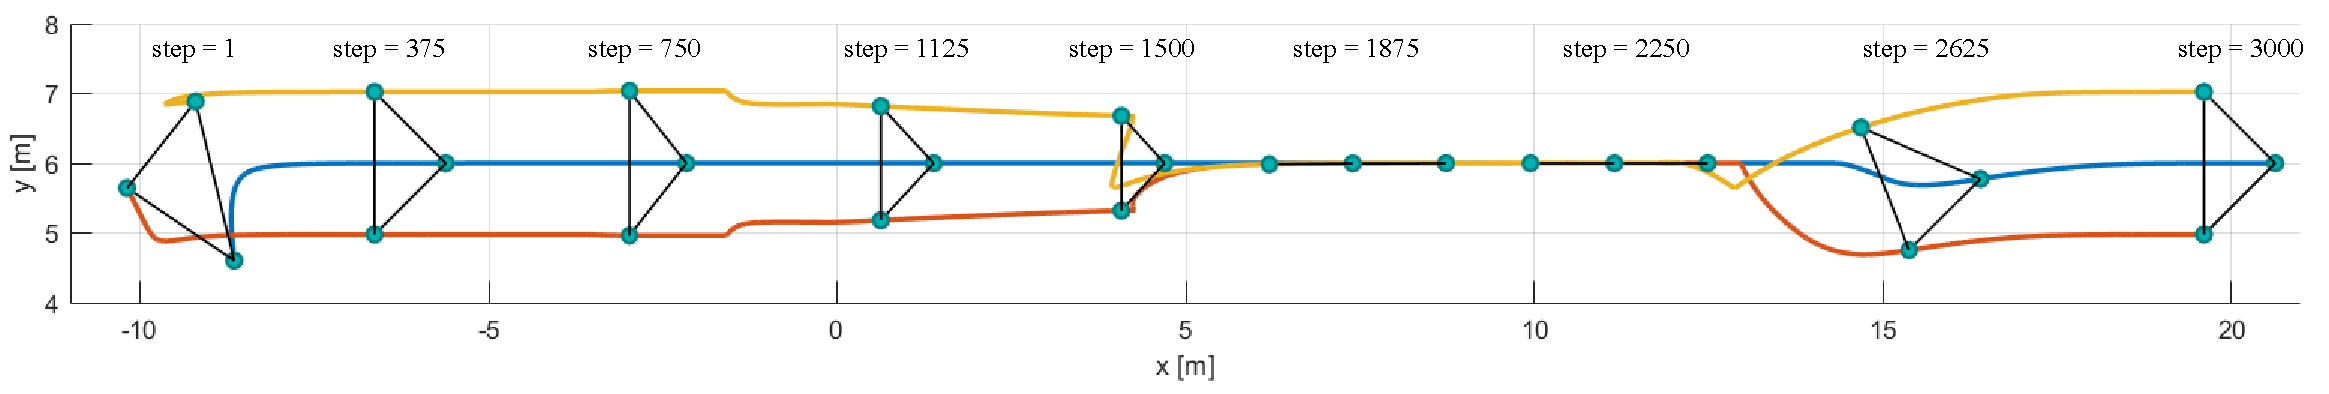
\includegraphics[width=\textwidth]{paper2/images/gazebo_path.pdf}
    \caption{The recorded paths of three UAV in the SIL test (Top view)}
    \label{fig:1gazebo_path}
\end{figure*}

To evaluate the applicability of the proposed system, we have conducted a software-in-the-loop (SIL) validation that involves navigating UAV formation pass through a confined space, which only focuses on a narrow tunnel-like environment in a Gazebo\footnote{Gazebo experiment video: {\fontfamily{qcr}\selectfont
\url{https://youtu.be/AIAAzRiIepg}}}. The used UAV model is a Hummingbird quadrotor developed based on Gazebo-based RotorS simulator~\cite{Furrer2016}, as described in Fig.~\ref{fig:1gazebo_uav}. We set up three UAVs in the experiment with random positions, as shown in Fig.~\ref{fig:1gazebo_init}. The environment in the SIL test includes two large obstacles, forming a width-varying tunnel, as depicted in Figure \ref{fig:1gazebo_env}.

Fig.~\ref{fig:1gazebo_result} presented the formation moving captured in the experiment. Moreover, the paths of three UAVs in the SIL test are recorded and are depicted in Fig.~\ref{fig:1gazebo_path}. At the beginning of the motion (step 1), three UAVs are in the random position. They then move to form the desired triangle formation (steps 375 - 750), as shown in Fig.~\ref{fig:1gazebo_1}. When sensing the narrow passage, the formation shrinks to safely move through the passage (steps 1125 - 1500), as shown in Fig.~\ref{fig:1gazebo_2}. When the narrow space is not suitable for the original formation, the formation transforms to the straight line formation as Fig.~\ref{fig:1gazebo_3} and then passes through the space with the line formation (steps 1875 - 2550), as Fig.~\ref{fig:1gazebo_4}. Once the UAV senses enough space in the environment to maintain its original formation, the formation transforms back to the origin shape in Fig.~\ref{fig:1gazebo_5} and moves to the target in Fig.~\ref{fig:1gazebo_6} (steps 2625 - 3000). The experiment demonstrates that the proposed \textit{EFRC} strategy successfully navigates the UAVs' formation to the target by passing through the narrow passage.

% \subsection{Discussion}
% Through simulation, validation, comparative statistics, and SIL testing, it is clear that our proposed method is capable of navigating the formation ensuring configuration, safety, and optimality for robot operation in narrow space environment.

% The proposed strategy provides flexibility for the robot formation to move safely through narrow space environments with numerous of formation configuration the ability to scale, rotate, and transform into a line configuration based on the perception of the environment depicted in Figure \ref{fig:1path}.

% The proposed algorithm also ensures scalability across various robot quantities within the formation, as presented in Figure \ref{fig:1path}. As long as the robots adhere to the specified configuration, the strategy offers the flexibility to navigate through narrow environments effectively.

% In our design, the formation maintenance and tailgating behaviors are proven to be stable through Lyapunov's theorem (see Appendix \ref{app:uf} and Appendix \ref{app:ut}), which proves that the system errors will converge to zero, as provided in Figure \ref{fig:1error}. Their convergence speed can be controlled through the parameters, $k_f$, $k_t$.

% On another note, our proposed strategy brings forth the capability to swiftly respond to environmental variations and traverse narrow spaces securely. Nonetheless, the transitions between states and abrupt alterations in formation size may result in occasional movement disruptions (see \textit{order} metric in Figure \ref{fig:1metric}). In such instances, employing control techniques like fuzzy logic or neural networks can be employed to improve the overall fluidity of formation movement.
\section{Conclusion}\label{sec5}
In this study, we have presented an event-based reconfiguration control to navigate a time-varying robot formation through narrow spaces across various environmental settings, including forest-like and tunnel-like terrains. The proposed strategy is constructed via several behaviors, which leverage the artificial potential field, which brings t to facilitate implementation. The controller includes two modes, \textit{``formation''} and \textit{``tailgating''}, and a scaling factor that enables the TVF to adapt its shape based on observed environmental conditions. The stability of the proposed approach is also demonstrated via the Lyapunov theorem. Evaluation results show that the proposed controller effectively navigates complex environments, achieving superior control performance in most metrics compared to other established methods. Additionally, software-in-the-loop tests verify the practicality and robustness of the proposed controller in real-world scenarios.

% \section*{Acknowledgement}
% Duy-Nam Bui was funded by the Master, PhD Scholarship Programme of Vingroup Innovation Foundation (VINIF), code VINIF.2023.Ths.088.

\balance

\ifCLASSOPTIONcaptionsoff
  \newpage
\fi

\bibliographystyle{IEEEtran}  
\bibliography{ref}
\end{document}